\scanpage{40}
\unsure{10)|19)} (Modulo the Hodge conjecture) $G^{\circ}$ is generated over $\unsure{\mathbb Q|Q}$ by $i_1^{\mathbb C}$.

\deleted{\unsure{10)} $G$}

% slanted
\margin{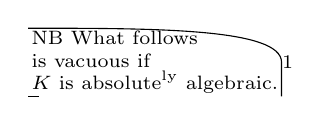
\begin{tikzpicture}[baseline=(current bounding box.north),font=\scriptsize]
\node[align=left,inner sep=1pt] (note) {\uline{NB} What follows\\is vacuous if\\$K$ is absolute\textsuperscript{ly} algebraic.};
\draw (note.north west) .. controls (note.north) and (note.north east) .. (note.east)
.. controls (note.east) and (note.south east) .. (note.south east);
\draw (note.south west) -- ([xshift=4pt]note.south west);
\node[anchor=west,inner sep=0pt] at (note.east) {\deleted{\illegible{1}}};
\end{tikzpicture}}
Let $R\subset G$ be the algebraic subgroup generated by $w(\pi_1(S(\mathbb C),\xi))$. It is \uline{normal} by \unsure{9)|4)} [for the closed image of $\pi_1(S(\mathbb C),\unsure{\xi|1})\relbar\pi_1(S,\xi)$\} is a normal subgroup\}, the quotient being $\pi_1(\operatorname{Spec} k,\xi)$, where $k$ is the algebraic closure of $\mathbb Q$ in $K$]. \deleted{The \unsure{composite}} By virtue of 4), the homomorphism
\diagram{\begin{tikzcd}[ampersand replacement=\&,column sep=1.4em,row sep=.5ex]
{} \& {} \& \inserted{\widetilde G(\mathcal A),\ \text{where }\widetilde G=G/R,}\\
\pi_1(S\unsure{\mathbb C|\in},\xi) \arrow[r] \& G(\unsure{\mathcal A|\mathscr A|A}) \arrow[ur] \& {}
\end{tikzcd}}
therefore factors as
\[
\tilde u:\underset{\substack{\Vert\\[-.4ex]\simeq\\[-.4ex]\unsure{\pi_1|\Vert}}}{\pi_1(\operatorname{Spec}(k),\xi)}
\longrightarrow\widetilde G(\mathcal A)
\]

On the other hand, one considers the torsor $\widetilde P=P/R$ under $\widetilde G$, with the integrable connection deduced from that of $P$. One has

\margin{\deleted{\uline{\illegible{1}}}}
\unsure{16)|18)|10)} \inserted{(Modulo Hodge)} $(\widetilde P,\widetilde G)$ with its integrable connection ``descends to $k$'', so one has a torsor $(\widetilde P_0,(\widetilde G/k)$ over $k$, and an isomorphism of torsors
\begingroup
\csname tagsleft@true\endcsname
\[
\widetilde P=P/R\simeq\widetilde P_0\otimes_k K \tag*{(*)}
\]
\endgroup

\deleted{Moreover, \deleted{setting} introducing $R'\subset G'$ corresponding to $R$, and $\widetilde G'=G'/R'$, so that one has an isomorphism}
\[
\deleted{\widetilde G'=\widetilde G'_0\otimes_k K,\qquad
\widetilde G'_0=\underline{\operatorname{Aut}}_{(\widetilde G/k)-}(\widetilde P_0),}
\]
\deleted{the subgroup \deleted{$\unsure{\widetilde H'|H'}\subset\unsure{\widetilde G'|G'}$} \inserted{$\widetilde H'=H'/H'\cap R'\unsure{=|\simeq}\operatorname{Im}(H'\longrightarrow\widetilde G')$} is ``defined over $k$'' i.e. comes from $\widetilde H'_0\subset\widetilde G'_0$}

\inserted{Finally the isomorphism \unsure{(*)|here}, $\unsure{\in|\xi}$ which} \deleted{The filtration structure on the functor $T$} defines, for a $\widetilde G$-module $M$, a descent structure on $P\mathbin{\times}^{G_K}M_K$ to $k$\unsure{,|;} [it is the one defined by the integrable connection of $P\mathbin{\alpha}^{G_K}M_K$], gives a descent datum \uline{compatible} with the filtration, i.e the latter is \uline{horizontal}, $\bigl[\!\bigl[$ thus \deleted{\illegible{1}} $\widetilde H'=\operatorname{Im}(H'\longrightarrow\widetilde G')$, $\widetilde Q,=Q\mathbin{\times}^{\unsure{H'|\widetilde H'}}\widetilde H'$, descend \unsure{respective\textsuperscript{ly}|respective\textsuperscript{ly}} to $\widetilde H'_0\subset\widetilde G'$ and a right torsor $Q_0$ under $\widetilde H'_0$, \unsure{\deleted{and}|and} (whence $\widetilde H''_0$ and $\widetilde G''_0$ which descend $H''$ and $\widetilde G''$), and \deleted{\unsure{after}} the composites $\tilde i_1,\tilde i_2:\mathbb G_m\underset K{\relbar}G''\longrightarrow\widetilde G''$ descend to $(\tilde i_1)_0,(\tilde i_2)_0:\mathbb G_{m\,k}\longrightarrow\widetilde G''_0$ $\bigr]\!\bigr]$.
% archive sheet number: 39
